
\section{Literature comparison}\label{sec:comparisons}
Given that the distance network is an extension of the distance ladder framework, it is only natural, and an important test, that we should be able to reproduce various literature results using this framework. A few caveats to this arise from the simplifications we made in order to build the distance network, as well as possibly different treatments of objects in the Hubble flow (e.g., different peculiar velocity treatments). However, these are not expected to cause significant differences ($\lesssim 0.3$ km\,s$^{-1}$Mpc$^{-1}$) in the final determination of \Hcst. 

\subsection{Literature Replication and Comparison for SNe~Ia\label{app:replication}}
Given the dominant role of the SNe~Ia in previous claims of a Hubble tension, we focus in this part of the appendix on the agreement of the SNe~Ia-derived results by exploring a broader range of SN Ia light curve fitters and SN Ia calibration samples than those included in the main variants Section~\ref{sec:variants} that may help explain the origin of differences in $H_0$ compared to literature studies. 
\begin{figure}
    \centering
    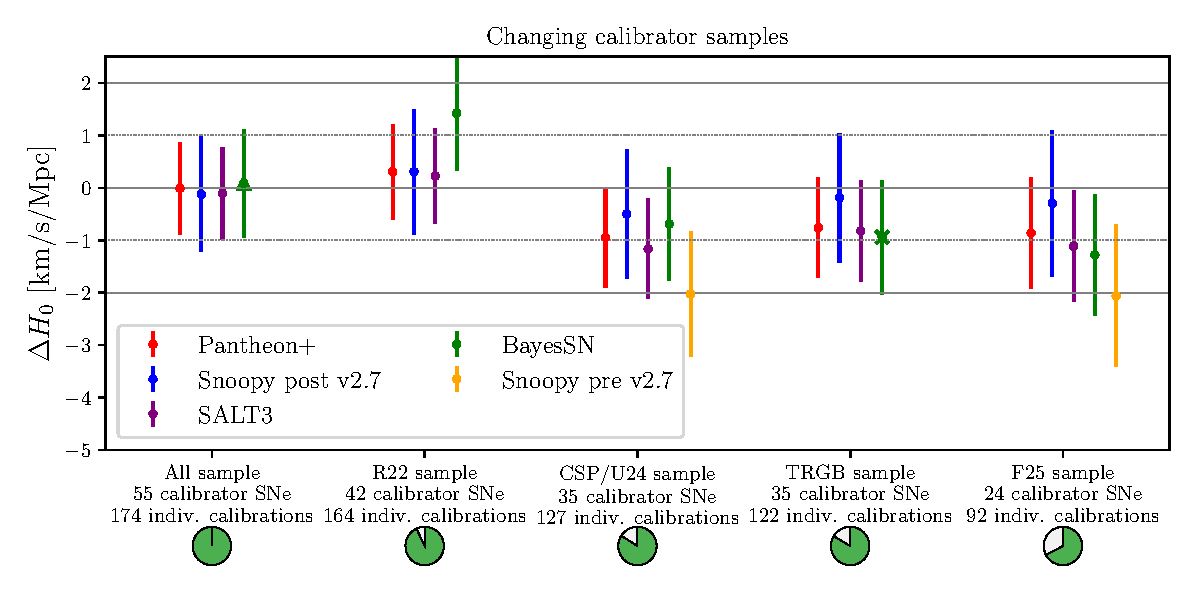
\includegraphics[width=0.9\linewidth]{Figures/sn1a_literature_v8.pdf}\caption{Comparison of the impact of supernova type Ia calibrator samples (sets of hosts) on the Hubble constant inference $H_0$\,, each one relative to the baseline result, for the various light curve fitting codes. The triangle shows a case where for the bayesSN fitter only 52 out of the 55 hosts was calibrated due to several missing supernovae in the fit, and the cross one where only 32 out of 35 hosts were calibrated. For details on the pie charts, see Fig.~\ref{fig:paths_consistency}. In this case we take 100\% of the pies to be the case involving all supernovae data instead of the baseline.}
    \label{fig:literature_sn1a}
\end{figure}

\begin{table}[h]
\begin{center}
\centering
\begin{tabular}{l c c c c c}
\hline
SN Sample/Calibration  (SN count) & Pantheon+ & SNooPy post v2.7 & SALT3 & BayesSN & SNooPy pre v2.7 \\
\hline
All/All (55) & $73.49 \pm 0.87$ & $73.37 \pm 1.10$ & $73.39 \pm 0.88$ & $(73.58 \pm 1.03)^{*}$ & --- \\
R22/All (42) & $73.80 \pm 0.91$ & $73.80 \pm 1.19$ & $73.72 \pm 0.91$ & $74.92 \pm 1.09$ & --- \\
R22/Cepheids (42) & $73.17 \pm 0.96$ & $73.33 \pm 1.23$ & $73.06 \pm 0.96$ & $74.67 \pm 1.14$ & --- \\
CSP in U24/All (35) & $72.54 \pm 0.95$ & $72.99 \pm 1.23$ & $72.33 \pm 0.95$ & $72.80 \pm 1.08$ & $71.47 \pm 1.20$ \\
CSP in U24/TRGB (27) & $71.61 \pm 1.53$ & $72.62 \pm 1.75$ & $71.50 \pm 1.52$ & $71.44 \pm 1.57$ & $70.99 \pm 1.70$ \\
TRGB HST-JWST/All (35) & $72.73 \pm 0.96$ & $73.31 \pm 1.23$ & $72.67 \pm 0.96$ & $(72.55 \pm 1.09)^{+}$ & --- \\
TRGB HST-JWST/TRGB (35) & $72.18 \pm 1.48$ & $72.66 \pm 1.64$ & $72.13 \pm 1.48$ & $(71.55 \pm 1.55)^{+}$ & --- \\
F25/All (24) & $72.63 \pm 1.06$ & $73.20 \pm 1.40$ & $72.38 \pm 1.06$ & $72.22 \pm 1.16$ & $71.44\pm 1.36$ \\
F25/TRGB (24) & $71.09 \pm 1.63$ & $72.05 \pm 1.85$ & $70.97 \pm 1.63$ & $71.00 \pm 1.66 $& $70.31 \pm 1.80$ \\
\hline
\end{tabular}
\caption{\label{tab:literature_sn1a}Comparison of Hubble constant values (in km\,s$^{-1}$Mpc$^{-1}$) from different supernova sets and calibrators. Note that for the same calibrator sets differences in the uncertainty stem mostly from the number of objects in the Hubble flow. SNooPy pre v2.7 is the one used in U24/F25. \\ {\footnotesize${}^{*}$ In this case only 52 out of the 55 calibrators could be matched with the given set of fitted SNeIa.}\\{\footnotesize${}^{+}$ In this case only 32 out of the 35 calibrators could be matched with the given set of fitted SNeIa.}}
\end{center}
\end{table}

First, we compare our distance network in the case that we only use type Ia supernovae as secondary distance indicators and in the Hubble flow. For this case, we can compare to three references, namely \cite{2022ApJ...934L...7R,2023MNRAS.524..235D,2025ApJ...985..203F}. This comparison is graphically summarized in Figure~\ref{fig:literature_sn1a} and Figure~\ref{fig:literature_sn1a_delta} , and the corresponding numbers can be found in Tables~\ref{tab:literature_sn1a} and \ref{tab:literature_other}. We observe that all comparisons agree between the publication and the \DN{} emulation within less than $0.15\sigma$ on the inferred value of $H_0$\,. In particular, when using only the 42 calibrators of \cite{2022ApJ...934L...7R} for Pantheon+ supernovae and adopting only the Cepheid calibration as in that study, we find $\Hcst = 73.17 \pm 0.96 \Hunit$ where they find $\Hcst=73.15 \pm 0.97\Hunit$ ($0.02\sigma$ difference, 1\% smaller uncertainty). Note that we compared to the results of \cite{2022ApJ...938...36R}, as the {\DN} also includes the cluster Cepheids that tighten the calibration in the anchors. When comparing to the Cepheid-based results of \cite{2023MNRAS.524..235D} based on BayesSN supernovae, we find in this case $\Hcst = 74.67 \pm 1.14 \Hunit$ where they find $\Hcst = 74.82 \pm 1.28 \Hunit$ ($-0.12\sigma$ difference, 11\% smaller uncertainty). In this case, there is an additional caveat that \cite{2023MNRAS.524..235D} only used 41 calibrators whereas with the BayesSN supernova fitter we used 42 Cepheid calibrators in this case. Finally, when comparing to the 24 TRGB-calibrated SN Ia results of \cite{2025ApJ...985..203F} (from HST or JWST), we find $\Hcst = 70.31 \pm 1.80 \Hunit$ where they find $\Hcst = 70.39 \pm 1.22 \mathrm{(stat)} \pm 1.33 \mathrm{(sys)} \pm 0.70 \mathrm{(\sigma_\mathrm{SN})} \Hunit$ ($-0.06\sigma$ difference, 0.3\% smaller uncertainty when comparing the relevant uncertainties in quadrature). We can also compare the values of the calibration in these cases, finding for \cite{2022ApJ...934L...7R} $M_B = -19.260 \pm 0.027$ ($-0.18\sigma$ compared to $M_B = -19.253 \pm 0.027$), for \cite{2023MNRAS.524..235D} $\Delta M_B = 0.039 \pm 0.027$ ($+0.4\sigma$ compared to $\Delta M_B = 0.030 \pm 0.023$, with one additional calibrator), and for \cite{2025ApJ...985..203F} $M_B = -19.186 \pm  0.053$ ($-0.11\sigma$ compared to $M_B = -19.18 \pm 0.04 \mathrm{(stat only)}$).  We thus take as a noteworthy conclusion that the DN can accurately reproduce the individual distance ladder results based on the host distances, standardized SN magnitudes, and geometric calibrations used in these studies.  

\subsection{Understanding differences in \texorpdfstring{$H_0$}{H0} for past SN Ia-based ladders}\label{app:sec:SNIa_literature}

Since we can reproduce the literature results within our framework, we can also investigate the sources of differences
in $H_0$ which may be attributed to specific analysis choices and datasets.  

\subsubsection{Refitting with new, SNooPy v2.7.0\label{app:snoopy}}
An immediate challenge to comparing and extending the SN Ia results that make use of the SNooPy fitter (used in all CSP and CCHP studies) is both the absence of many useful SN calibrators in the \citet{2024ApJ...970...72U} (hereafter U24) the compilation that was used in \cite{2025ApJ...985..203F} (hereafter F25) as well as the update to the SNooPy fitter to version v2.7.0 or later (since Aug 27, 2024)-- with the prior version which we dub ``pre v2.7'' (the prior release was 2.5.3 Jan 29, 2020) that was used in U24 not readily accessible nor recommended for further use by its author.  According to C. Burns who supports SNooPy development (private communication, 2025) current studies are advised to use the latest, v2.7.0.  The most relevant update in v2.7 involves the method used by SNooPy to extrapolate the light curve templates beyond the training sample ($s(B-V) < 0.3$ and $s(B-V) > 1.27$).
Such SN Ia have light curves and inferred luminosities near the extrema of the distributions (often going by the name ``91bg-like'' at the faint and fast side and "91T-like" at the bright and slow/high stretch side).  This has very little affect on the calibrator sample (which are often pre-selected to be normal or near the middle of the distribution, see R22).  However, the Hubble flow sample, and specifically the CSPII sample has a surprising abundance of ``high-stretch'' or 91T-like SNe Ia (U24). We find $18$ supernovae in CSPII and $5$ in CSP I (so 23 in all).  Such SNe Ia will generally have $s(B-V) \geq 1.15$ for which the impact from the version update is quite large.
The prior SNooPy version (pre v2.7) was found to over-correct these, motivating the revision to the fitter. For the updated SNooPy v2.7, prior fits with $s(B-V) \sim 1.15$ are lowered on average to $s(B-V) \sim 1.0$ (the fitted, apparent peak magnitudes are hardly impacted) and the implied reddening in $B-V$ is increased by $\sim$ 0.04 mag. The net change comparing old and new follows as $\Delta m \approx 0.9 \cdot (1.15-1.0)-2.9 \cdot(-0.04) \approx 0.25$ mag (neglecting a small quadratic term in $s(B-V)$ for this illustration) for the high $s(B-V)$ supernovae with the new standardized magnitude being brighter (since a brightness previously attributed to over-luminosity and low extinction is now reflected in the newly, brighter standardized magnitudes). Specific examples which all have $s(B-V)>$1.1 include CSP12G, CSP13Z, CSP13aad, LSQ12agd, LSQ12gef, LSQ12hxx, LSQ13dqh, and PTF14uo which all change by 0.2-0.3 mag in the same, brighter direction.  As 91T's represent $\sim$ 8\% of the CSP sample, we might expect a mean change of $\sim$ 0.02 mag which is similar to the actual change from the new version of $\sim$0.03 mag (which includes error weighting).  This appears as an increase in the Hubble flow intercept of $a_B=0.6843\pm0.0025$ to $a_B=0.6895\pm0.0026$ $(+2\sigma)$. As a result $H_0$ increases by 1.0 km\,s$^{-1}$Mpc$^{-1}$ due only to the change in the measurement of the Hubble flow for CSP from the new SNooPy.

An independent consideration is that it is also necessary to use the newer SNooPy v2.7 to fit additional SN Ia calibrators not included in the U24 compilation produced from pre v2.7 SNooPy.  New SNooPy v2.7 fits were thus made by C. Burns (private communication, 2025) using the versions of the light curves in the Pantheon+ light curve database, most of which are not CSP light curves.  In the process a number of discrepancies were identified from the prior SNooPy fits in U24 and \citet{2019ApJ...882...34F} (hereafter F19).  These were either the use of an older data release when a newer and better one was available (e.g., \texttt{Cfa I} from \citet{1999AJ....117..707R} did not employ host subtraction which was applied and released in \citet{2005ApJ...627..579R,2007ApJ...659...98R}), an inconsistency in a filter function definition (i.e., when older published data were provided after transformation to the Landolt/Bessel system, not the ``natural'' system, e.g., 1998bu and 2002fk)  or the use of a broader set of optical light curves was available. 

These differences tend to pertain to older light curves from \texttt{CfA I} or \texttt{LOSS}, with changes in either direction, as tabulated in Table~\ref{table:choice_data}. 

\begin{table}[h!]
\centering
\caption{Differences in SN~Ia lightcurve data adopted in F19/U24/F25 compared to the best available data.}
\begin{tabular}{lllll}
\hline
\hline
SN & Used in F19/U24/F25 & Best Available & Improvement & Difference $\Delta B_{corr}$\\
\hline
1992A  (Cfa I)      & Suntzeff (1996)   & Suntzeff (1996)    &  fit to UBVRI (not BV) &  $0.08$ \, mag \\
1994ae (Cfa I)      & \citet{1999AJ....117..707R}$^{(a)}$ & \citet{2005ApJ...627..579R}   &  host subtraction, 4x phot cal. &  $0.02$ \, mag \\
1995al (Cfa I)     & \citet{1999AJ....117..707R} & \citet{2009ApJS..183..109R}   &  host subtraction, 4x phot cal. &  $0.29$ \, mag \\
1998bu (Cfa I)      & \citet{1999ApJS..125...73J} & \citet{1999ApJS..125...73J}   &  filter function &  $0.25$ \, mag \\
2002fk (LOSS)      & \citet{2009ApJS..183..109R}  & \citet{2009ApJS..183..109R}    &  filter function &  $-0.06$ \, mag \\
2012cg (LOSS) & \citet{2016ApJ...820...92M}  & \citet{2019MNRAS.490.3882S}    & final reduction  & $-0.28$ \, mag \\ 
2005cf (LOSS) & Open Source Catalogue &  \citet{2019MNRAS.490.3882S} & final reduction & $-0.06$ \, mag \\ 
2005cf (LOSS) &  Open Source Catalogue & \citet{2019MNRAS.490.3882S} & final reduction & $-0.04$ \, mag \\ 
2013dy (LOSS) &  Open Source Catalogue  & \citet{2019MNRAS.490.3882S}  &  final reduction  & $0.35$ \, mag \\ 
2017cbv (LOSS) & Open Source Catalogue & \citet{2019MNRAS.490.3882S} &  final reduction & $-0.10$ \, mag \\
2011fe  & \citet{2012JAVSO..40..872R} & LOSS &  coverage &  $0.04$ \, mag  \\
\hline
~ \\
\end{tabular}
\label{table:choice_data}
\tablecomments{$^{(a)}$ Reference F19 claims that 1994ae used the version of the light curve from  \citet{2005ApJ...627..579R} , but C.~Burns, who performed the fit, sourced the data from the Open Source Catalogue, which instead used \citet{1999AJ....117..707R}.  We further confirm that the value in \citet{2024ApJ...970...72U} matches \citet{1999AJ....117..707R}, not \citet{2005ApJ...627..579R}}
\end{table}

Due to the rarity of NIR light curves for calibrators which span decades and require data before NIR observations were common, to avoid introducing a systematic error (from the difference between optical and NIR calibration) we did not include NIR data for the CSP Hubble flow (in practice we found this difference is negligible). See however \ref{sec:variant_description} for variants that specifically use only NIR information for both calibrators and Hubble flow.

The net change from SNooPy pre-v2.7 to post-v2.7 makes the mean calibrator fainter in $M_B$ by 0.026 mag for the F25 sample of $24$ SNeIa and 0.019 mag for the full in-common sample of $35$ SNeIa. {\bf Overall, compared to prior SNooPy fits, the fits of the current version (SNooPy v2.7) raise $H_0$ for the same SN samples by $\mathbf{\sim1.7\,\mathbf{km \, s^{-1} \, Mpc^{-1}}}$ (e.g., from 70.31 for the F25 sample to 72.05).}  This difference is caused then primarily from improvements to SNooPy and to a lesser degree from better, later versions of the SN Ia calibrator data, see Table~\ref{tab:snoopy}.

\begin{table}[h!]
\centering
\caption{Dependence of $H_0$ on SNooPy Fitter version and SN Sample for TRGB Ladder\label{tab:snoopy}}
\begin{tabular}{lcc}
\hline
Result/difference &  \textbf{$H_0$} & \textbf{Notes} \\
\hline
F25 (SNooPy pre v2.7, F25 sample) & ${\bf 70.39} \pm 1.80$ ($N=24$) & F25 as published (without additional SN calibration error) \\
\,\,\,\,\,\,  \rotatebox[origin=c]{180}{$\Lsh$} No change to SNooPy version or sample & $70.31 \pm 1.80$ ($N=24$) & Reproduced within our network \\
\,\,\,\,\,\,  \rotatebox[origin=c]{180}{$\Lsh$} SNooPy post v2.7, F25 sample & $72.05 \pm 1.85$ ($N=24$) & New SNooPy raises $H_0$ \\
\,\,\,\,\,\,  \rotatebox[origin=c]{180}{$\Lsh$} SNooPy pre v2.7, all available pre v2.7 sample & 71.40 $\pm 1.72$ ($N=28$) & SN in U24 not included in F25 raises $H_0$ \\
SNooPy post v2.7, all available post v2.7 sample &  ${\bf 72.66}\pm 1.64$  ($N=35$) & combination, new SnooPy+all SNe with TRGB \\
\hline
\end{tabular}
\vspace{2mm}
\parbox{0.9\linewidth}{\footnotesize \textit{Note.} Differences with F25 for Same Ladder ,  NGC 4258 $\rightarrow$ HST+JWST TRGB $\rightarrow$ CSP SN Ia w/ SNooPy

SNooPy pre v2.7 is from Uddin+24 and also limited to sample available there.  SNooPy post v2.7 includes current version of SNooPy with refits of best data versions by C. Burns as described in text. There is no difference in peculiar velocity treatment across entries.}
\end{table}

\subsubsection{Differences with Calibrator Sample Size}

Lastly, within the use of every SN fitter, increasing the sample size from the smallest, selected study (the F25 sample of 24 calibrators) to the full available sample of 55 calibrators shows a clear trend towards increasing $H_0$---as evident from Figure~\ref{fig:literature_sn1a} and Table~\ref{tab:literature_sn1a}. It increases by $0.9\Hunit$ for Pantheon+ fitting, by $0.2\Hunit$ for SNooPy post-v2.7 fitting, by $1.0\Hunit$ for Salt 3 fitting, and by $1.4\Hunit$ for BayesSN fitting---a mean of $+0.9 \Hunit$. This difference due to calibrator sample is even greater between the F25 sample and that from R22, about $1.2 \Hunit$ in the mean, agreeing with the findings of \cite{2024ApJ...977..120R}. This is shown in Figure~\ref{fig:literature_sn1a}. It seems reasonable to expect greater convergence in estimates of $H_0$ as sample sizes increase.

We note that the F25 sample is not a natural sample selection from the perspective of the \DN{}---it cannot be constructed from simple cuts in redshift/distance or calibrator type. As such, we do not consider it as a variant (according to the methodology laid out in Section~\ref{sec:select_variants}, those should be based on physical assumptions or hypotheses). We analyze it here to provide for a direct comparison with \citet{2025ApJ...985..203F}. We show the distribution in distance of the F25 ($N=24$) and full samples ($N=55$) according to the network in Figure~\ref{fig:mu_sample}---which shows that 37 of the 55 objects would have to be included if a cut was made in distance modulus to retain the full F25 sample. The smaller F25 sample is at a mean distance moduli of $\mu_\mathrm{host} = 31.13 \pm 0.85$, and the remaining sample is at a mean distance moduli of $\mu_\mathrm{host} = 32.01 \pm 0.73$, which are thus a little further away on average (though not very significantly). 

\begin{figure}
    \centering
    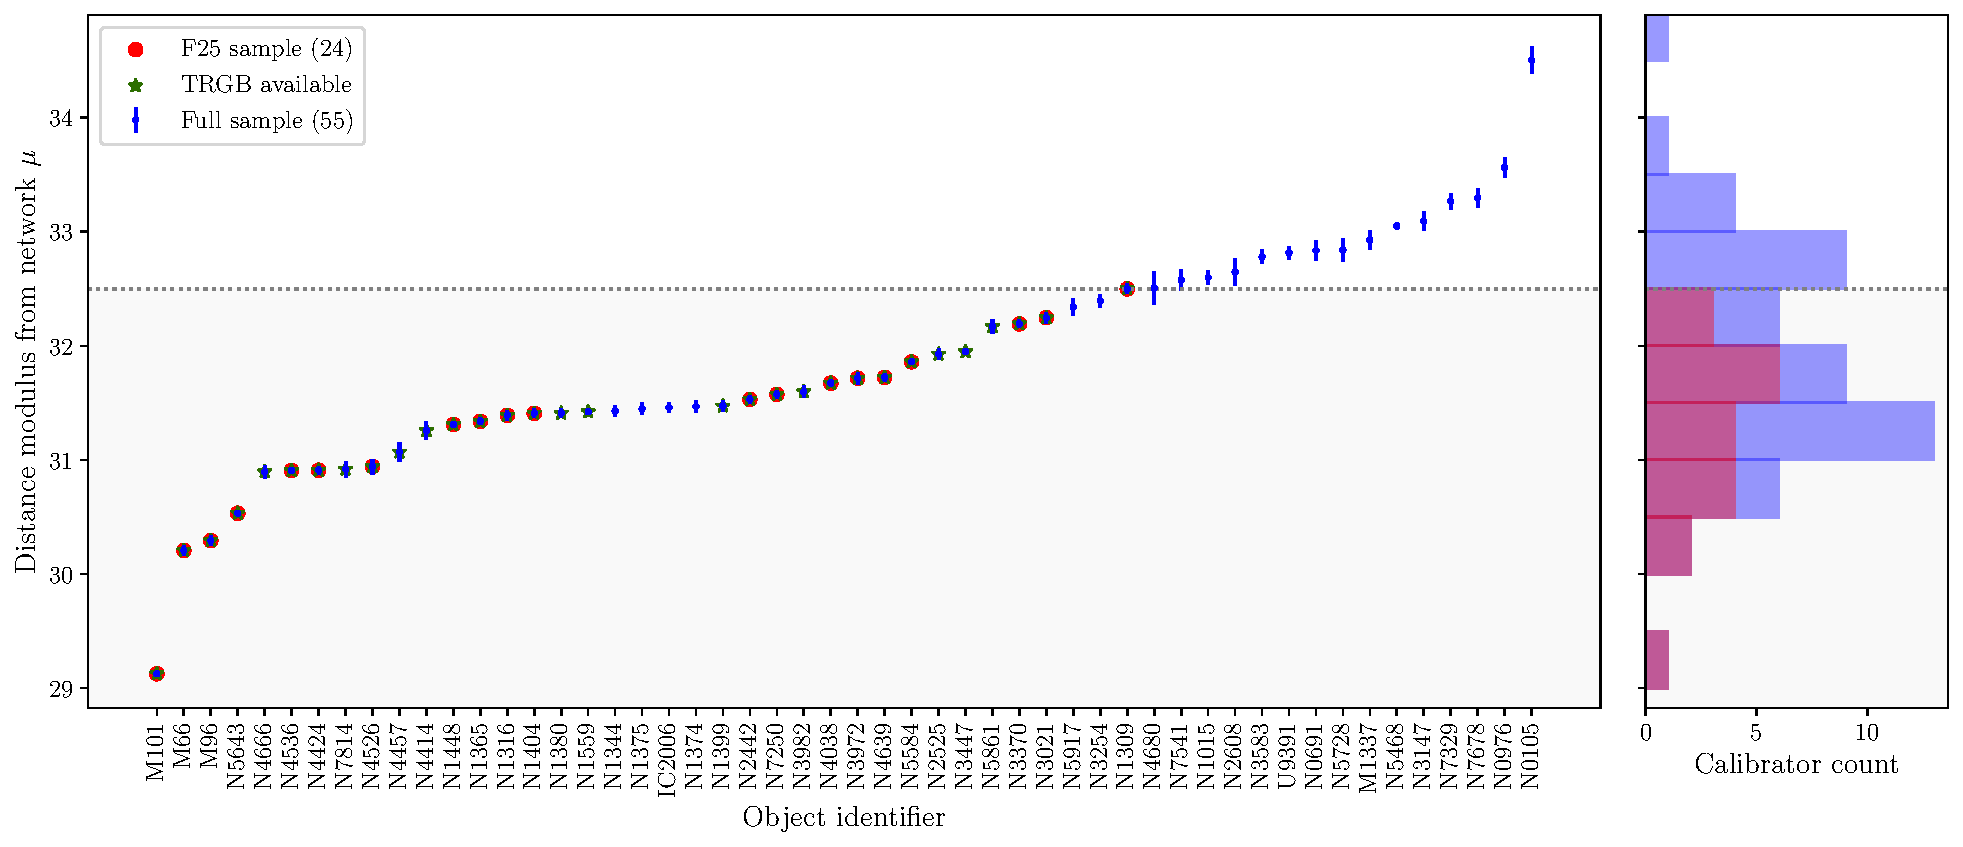
\includegraphics[width=0.95\linewidth]{Figures/mu_selection_v2.pdf}
    \caption{The full network sample (blue) and the F25 sample of calibrator hosts (red) in comparison. The grey region marks the maximal extent of the F25 sample. The green stars mark hosts with TRGB distances available. The left hand side shows an ordered scatterplot of the distance moduli, while the right hand side shows the corresponding histogram. Note that while F25 calibrates 24 SN~Ia, these are located in only 20 hosts (hence only 20 points are marked red). The 11 additional hosts marked with green stars would correspond to potentially 10 additional SNe~Ia (with the 11th host NGC 1399 calibrating SBF, not SNe~Ia). One additional SN~Ia (2021pit) is present in an already F25-calibrated host (N5643) but not within the CSP sample. In total that makes 24+10+1=35 calibrators that are available for SNe~Ia calibrated through TRGB. Even within the sample of the CSP I\&II supernovae only, there would still be 4 additional CSPI\&II calibrators to be gained using TRGB observations of nearby hosts within the range of the F25 sample---with 7 additional TRGB-calibratable SNe~Ia not present within the CSP I\&II samples. The 4 ``missing'' TRGB-F25 calibrators are 2012ht in NGC~3447, 1998aq in NGC~3982, 1992A in NGC~1380, and ASAS14-lp in NGC~4666.}
    \label{fig:mu_sample}
\end{figure}

For this purpose we can also look at Figure~\ref{fig:literature_sn1a_delta}, which shows the differences between calibrator sets for the same supernovae standardizations and datasets. In each case we take the same supernovae to be used for calibration, but vary with which primary distance indicators the distances to their hosts are calibrated, for example using only HST Cepheids vs using all methods, or using only the TRGB (JWST and HST) vs using all methods, or using only the TRGB calibrations adopted in F25 vs using all methods. These differences are typically compatible with the uncertainty at $\sim 1\sigma$, with shifts around $-1\Hunit$ in central value. We also see that the reduced calibrations agree nicely with the results reported in the literature.

\begin{figure}
    \centering
    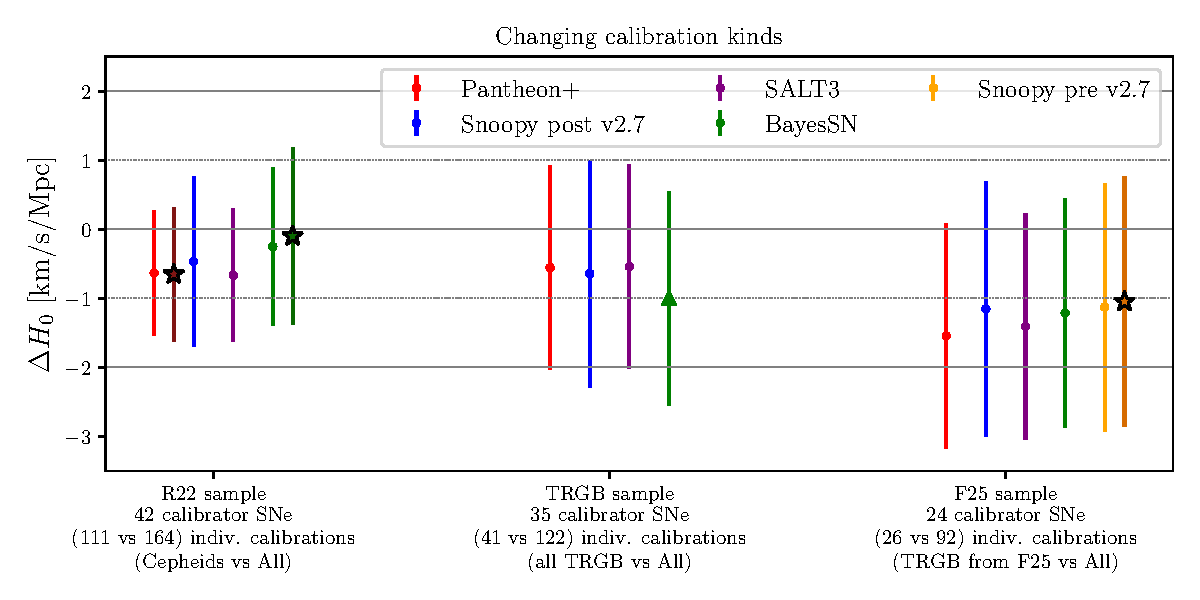
\includegraphics[width=0.7\linewidth]{Figures/sn1a_literature_part2_v5.pdf}
    \caption{Comparison of $H_0$ between different ways of calibrating a given set of hosts and a gievn SN fitter. It is computed as the result with the hosts calibrated through any means minus the result with the hosts calibrated through a specific calibration type (such as only Cepheids, only TRGB, or only F25 TRGB). The results with the star mark the literature results for the given (reduced) set of calibrating a given set of hosts. The triangle shows a case where for the BayesSN fitter only 32 out of the 35 hosts were calibrated due to several missing supernovae.}
    \label{fig:literature_sn1a_delta}
\end{figure}

\subsection{Literature comparison for other distance indicators}

Next, we compare our distance network to the case where we use other distance indicators. The results can be found in Figure~\ref{fig:literature_other} and Table~\ref{tab:literature_other}. These results are generally very consistent with the literature results, deviations typically staying at $0.1\sigma$ or less, once the same configuration is enforced. 

The SNII standard candle method naively appears to give discrepant results ``out-of-the-box'' in the distance network compared to the results from \citet{2022MNRAS.514.4620D}. However, this is due to the change in calibration described in Appendix~\ref{sec:data:snii_SC}, where we only use 9 out of the 13 possible supernovae as described in that appendix. If we adopt the precise calibration of \citet{2022MNRAS.514.4620D}, we recover their value very closely. For the megamasers of \citet{2020ApJ...891L...1P}, we recover the value without any changes. However, it is important to compare with the correct value, as our baseline employs 2M++ velocity corrections, and does not include N4258 as a non-anchor megamaser. For surface brightness fluctuations (SBF), it is important to correct the literature value for the impact of peculiar velocities manually, which we do by using the difference from peculiar velocities from \citet{2021ApJ...911...65B} (which is $\Delta H_0 = + 0.27 \Hunit$) and applying that to the value of \citet{2025MNRAS.539.3627S}, correcting the central value from $73.9$ to $74.17\Hunit$. We assume no further changes in the uncertainty. For the astrophysical modeling of type II supernovae (using the tailored expanding photosphere method (EPM)), we can directly reproduce the literature value within great agreement. For the Coma-derived value we check both values derived using only the SBF calibration or using only the supernovae from \citet{2022ApJ...934L...7R}. In both cases the result has excellent agreement with the literature value. Finally, we note that we did not manage to recover the literature value of the Tully-Fisher relation, but private communication with P. Boubel revealed that there might have been an issue in their code, leading to an incorrect value.  This only affects \cite{2024MNRAS.531...84B}; future work will be based on the data in earlier publications, which were not available to us at the time of this analysis.

\begin{figure}
    \centering
    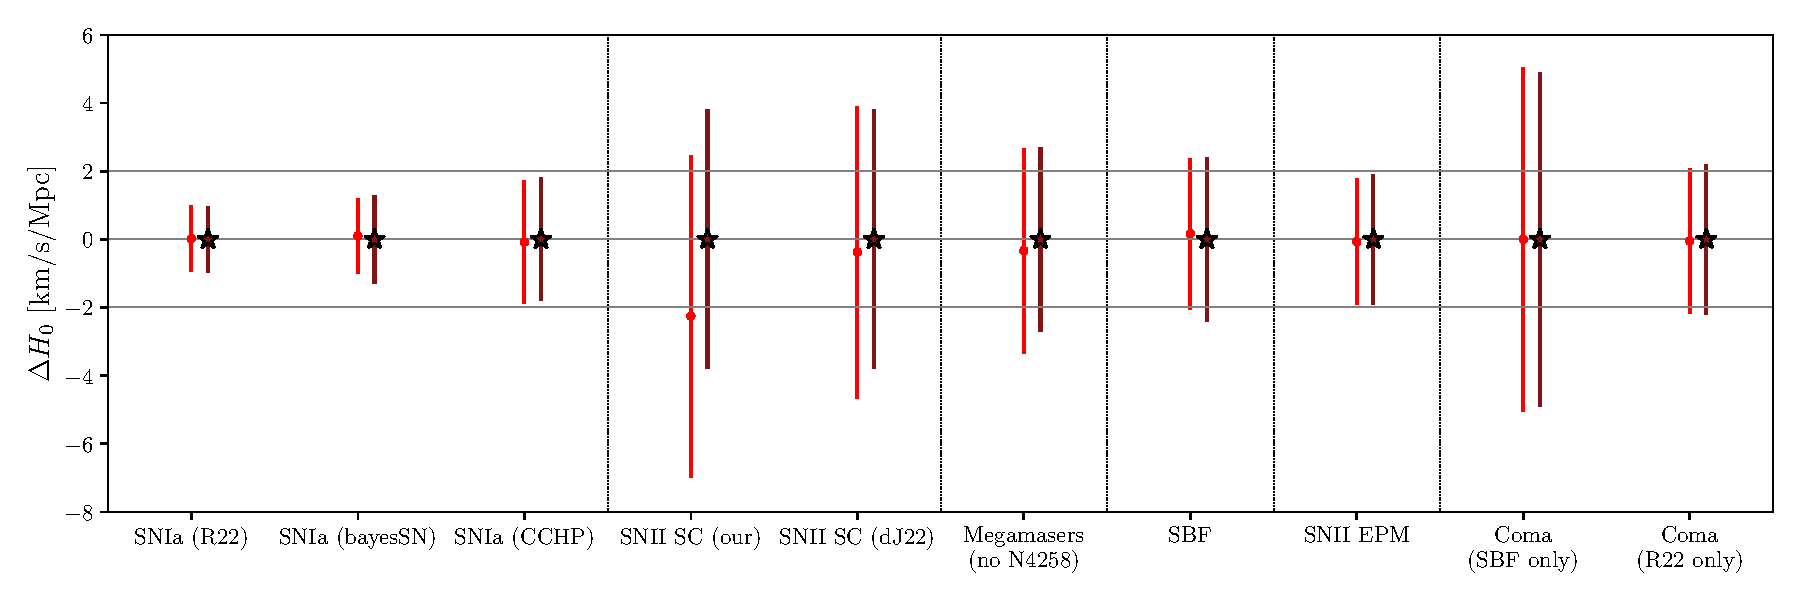
\includegraphics[width=0.95\linewidth]{Figures/rest_literature_v4.pdf}
    \caption{All literature comparisons for the given configuration/method (see x-axis label and main text). The light red results are the results for the given configuration/method coming from the {\DN}, while the dark red results are those available in the literature (differences are always zero but illustrates literature uncertainties), see also Table~\ref{tab:literature_other}.}
    \label{fig:literature_other}
\end{figure}

\begin{table}[h]
\caption{Comparison between Recent Literature Results and DN Emulation with the Same Data}
    \centering
    \begin{tabular}{l|l l c}
       Configuration  & Literature & Reference value & Our (DN) value \\ \hline
       SNIa (Pantheon+, R22 sample) & \citet{2022ApJ...938...36R} & $73.17\pm0.96$ & $73.15 \pm 0.97$ \\
       SNIa (BayesSN, R22 sample) & \citet{2023MNRAS.524..235D} & $(74.92 \pm  1.09)^{*}$ & $74.82 \pm 1.28$ \\
       SNIa (SNooPy pre v2.7, F25 sample) & \citet{2025ApJ...985..203F} & $70.31\pm1.80$ & $70.39 \pm 1.80$ \\
       SNII standard candle (SC), our calibration & \citet{2022MNRAS.514.4620D} & $75.4^{+3.8}_{-3.7}$ & $73.14 \pm 4.72$ \\
       SNII standard candle (SC), literature calibration & \citet{2022MNRAS.514.4620D} & $75.4^{+3.8}_{-3.7}$ & $75.02 \pm 4.29$ \\
       Megamasers (no N4258, 2M++ velocities) & \citet{2020ApJ...891L...1P} & $72.1 \pm 2.7$ & $71.77 \pm  3.01$ \\
       SBF (corrected) & \citet{2025ApJ...987...87J} & $74.17 \pm 2.40$ & $74.33 \pm  2.22$ \\
       SNII EPM & \citet{2025AA...702A..41V} & $74.9 \pm 1.9$ & $74.83\pm1.85$ \\
       DESI Fundamental plane (Coma via SBF-TRGB) & \citet{2025MNRAS.539.3627S} & $76.05 \pm  4.90$ & $76.05 \pm 5.05$ \\ 
       DESI Fundamental plane (Coma via SN-Cepheid)& \citet{2025ApJ...979L...9S} & $76.5 \pm 2.2$ & $76.45 \pm  2.13$ \\ 
    \end{tabular}
    \caption{Comparison of literature values with non-SNIa determinations of the Hubble constant from the distance network.\\{\footnotesize${}^*$ In this case only 41 out of the 42 SNe~Ia were fit in the reference.}}
    \label{tab:literature_other}
\end{table}

